%
% mountain.tex
%
\renewcommand{\thisname}{Chart::Mountain}
\section{\thisname}
\name{\thisname}
\file{Mountain.pm}
\requires{Chart::Base, GD, Carp, FileHandle}
\begin{Description}
The class \thisclass creates a mountain chart, \ie, the individual data
sets are stacked and the areas under the curves are colour filled.
The first data set will be shown at the top of the stack, the last at
the bottom. \thisclass is a subclass of Chart::Base.
\end{Description}

\example
\begin{figure}[ht]
  \begin{center}
    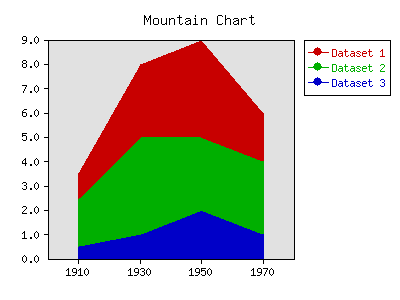
\includegraphics[scale =0.6]{mountain.png}
  \end{center}
  \caption{Mountain chart}
  \label{fig:mountain}
\end{figure}
\begin{verbatim}
use Chart::Mountain;

$g = Chart::Mountain->new();

@data = [ [1910, 1930, 1950, 1970],
          [1, 3, 4, 2],
          [2, 4, 3, 3],
          [0.5, 1, 2, 1]];

$g->set('title'      => 'Mountain Chart',
        'grid_lines' => 'false',
        'precision'  => 1);

$g->png("mountain.png", @data);
\end{verbatim}

\constructorblurb{\thisname}

\begin{AttrDecl}{y\_axes}
Tells \thisclass where to place the $y$ axis. Valid
values are \literal{left}, \literal{right} and \literal{both}. Defaults
to \literal{left}.
\end{AttrDecl}
